\documentclass{neu_handout}
\usepackage{url}
\usepackage{amssymb}
\usepackage{amsmath}
\usepackage{marvosym}
\usepackage{graphicx}
\usepackage[pdftex]{graphicx}
\usepackage{subfigure}
\graphicspath{ {images/} }
\everymath{\displaystyle}

% Professor/Course information
\title{A Bayseian Approach to Fake News}
\author{Emily Dutile, Shubhi Mittal, Linghan Xing}
\date{December 2017}
\course{CS5100}{Foundations of AI}

\begin{document}
\section*{1 Introduction and Background}

"Fake news" became an increasingly coined term and was almost non-existent in the general context and media providers prior to October 2016 of the Presidential Election. In late 2016, the top 20 fake news stories on Facebook were reported to outperform the top 20 real news stories, which was determined by the number of comments, reactions, and shares. As seen in figure a, it is shown that the number of real news stories did not outperform the number of fake news stories towards the end of 2016. Undoubtedly, these stories and articles our shaping and influencing the thoughts and opinions of millions of individuals and companies need to step in to help stop the spread of fake news.
\\\\
With companies such as Facebook and Google who provide ad revenue to sites that host news stories, it should be the responsibility of these tech companies to be accountable for what content is displayed. Filtering out false information in order to correctly inform and educate our society, especially when it comes to presidential elections, is an extremely important and challenging task. Companies such as Signal Media have built AI-powered media monitoring in order to help this problem after they had discovered 'fake news' as being a headline in 27,000 articles over the course of the year (see figure b).

\begin{figure}[h]
\centering
\subfigure[BuzzFeed News]
{
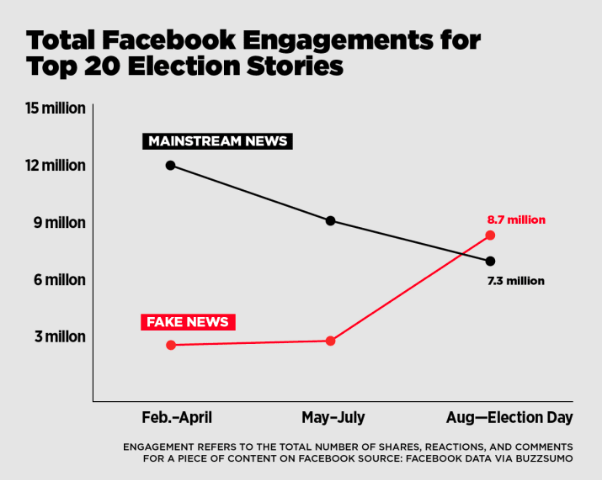
\includegraphics[width=0.3\linewidth]{buzzfeed}
}
\subfigure[]
{
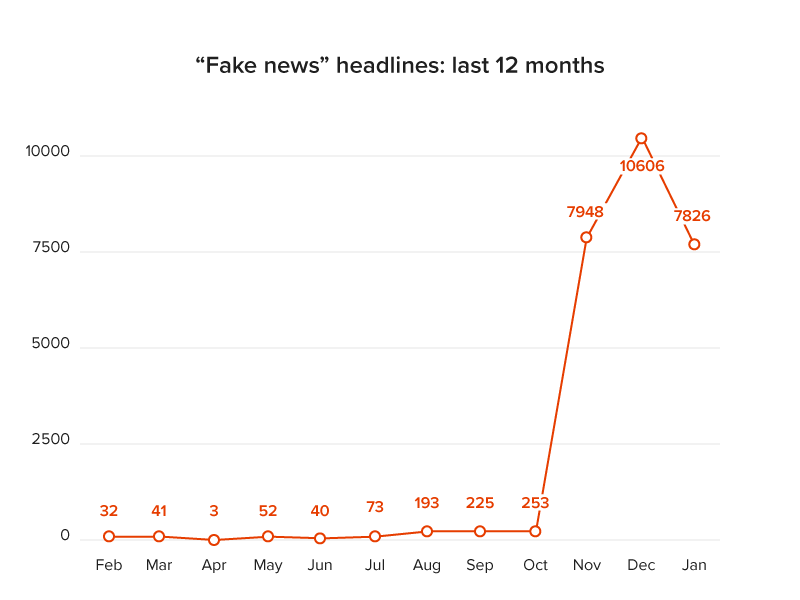
\includegraphics[width=0.3\linewidth]{fakenews}
}
\end{figure}

Fake news posts have exploited the feeds of Facebook users' which could deeply impact the options of our society if we loose our ability over time to decipher fake news from real news. Due to this problem, the data science community has looked to respond to this problem through a Kaggle competition called the Fake News Challenge \footnote{\url{http://www.fakenewschallenge.org}}. Determining real news from fake news is an extremely challenging task within the machine learning and natural language processing community. Creating models that accurately filter out fake news without removing real news sources is a very complicated task due to how we define fake news itself in order to correctly label real and fake news. 
\\
In our approach to tackle this problem, we wanted to combat fake news by implementing bayesian models that can differentiate fake news from real news. Expanding on this original approach, we have implemented several supervised machine learning based algorithms in order to compare text classifiers on fake news recognition. 


\subsection*{1.1 The Data}
As mentioned previously, what makes this challenge interesting and hard is around the very definition of fake news. Since we did not want to be caught up in the process of deciphering, scraping the web, and labeling fake news vs. real news, we found a dataset that contains almost 11,000 articles that are tagged as either real or fake news \footnote{\url{https://github.com/GeorgeMcIntire/fake_real_news_dataset}}. The data set seems to follow the definition of fake news provided by First Draft News comprises of 7 types of fake content: false connection, false context, manipulated content, satire or parody, misleading content, imposter content, and fabricated content. We started by separating the labels and set up training data and testing data.


\subsection*{1.2 Methods}
We performed supervised machine learning techniques such as naive bayes, multinominal bayes with count vectorizor (bag-of-words) and Term Frequency–Inverse Document Frequency (TF-IDF), along with SVM and Random Tree Forest. With respect to language processing, tokenization, filtering, lemmatization, and stemming were all used for preprocessing the titles and body text of the articles in the data set. For our evaluation process, we used a confusion matrix to understand the accuracy of our models.

\subsection*{1.3 Related Work}
Within the industry, companies such as Facebook have stumbled in this combat, mostly relying on users reporting fake news and outsourcing this task to third parties in order to remove direct bias. Although Facebook has made a few attempts and run some tests, it's clear that this is no easy task and can certainly annoy users.

\begin{figure}[h]
\centering
{
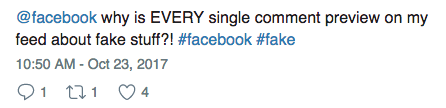
\includegraphics[width=0.3\linewidth]{fbfake}
}
\end{figure}

Some of the top teams that participated in the Fake News Challenge ended up using neural networks to get the best results. The number one team, SOLAT in the SWEN\footnote{\url{https://github.com/Cisco-Talos/fnc-1}}, received the best results using a weighted average between gradient-boosted decision trees and a deep convolutional neural network. Looking at the models that many teams had to take in order to receive the best results, we were not expecting our naive bayes model to product great results.

\section*{2 Supervised Approach}

\subsection*{2.1 Feature Extraction}

For feature extraction, we used the body text of the articles in the data set and ignored the titles. We thought that using the longer text would allow for distinct words and features from the data set. For understanding if the words and tokens in the articles text had a significant impact on whether the news was fake or real. 
\\
Given a list of documentations, feature extraction converts each of the documents into a list of features, generating a sparse matrix for our Naive Bayes model. Features from our text classifier could include anything from manually created labels to the occurrence of words in the texts. In our case the naive assumption is that given that fact that a document is fake or authentic, the occurrence of each word is independent from each other. To implement our feature extraction, we first extracted words from the documents/text. To do this, we used stop words, tokenization, and stemming.
\\
English stop words were removed from the data for better results. Stop words are frequent in our natural language but usually doesn't have additional information, such as words like "a", "on", "this", "the", "is", etc. By removing them the distraction in the vocabulary is usually reduced. In tokenization, the document is tokenized into a list of words, with all the punctuation being taken away and making all words lower case. In stemming, the words that have the same roots are assigned to the same root word. For example: "attack", "attacking" and "attacked" will be categorized as the same root word, "attack".

\subsubsection*{2.1.1 Count Vectorization}

After the word list for each document is built, a vocabulary can be established by looping through the documents and finding the set of words that occurred. This is often referred as "bag-of-words". Until this point, we have 'sanitized' our input text and can start building the count vector. There are two approaches that we implemented to get the term frequency matrix: naive boolean term frequency and logarithmic term frequency. The naive boolean term frequency is the simple way of counting the occurrence of each word in the vocabulary and simply assigning their occurrences in the matrix. This method is easier to implement and in many case yields reasonable results. In the second approach, we assume that the correlation between how important a word is a how many times the word occurs in the text should not be linear. If the word "love" occurred 4 times in a text, this does not mean that the author "loves" 4 times more than one who only used "love" once in their text. Therefore a possible improvement to that is to use logarithmic occurrence:
$$Frequency(w,d) = 1 + log(word_count)$$
 
To compare the results of our implementation, CountVectorizer was also used from the scikit-learn package and in this stage no weighting is assigned to any of these words.


\subsubsection*{2.1.2 TF-IDF}
In addition to the counting of term frequency, some words will occur very frequently in the documents to a point hat the occurrence of them does not provide much additional information. For example, if the word "American" is present in every text, then the occurrence of this word does not provide any information for our classifier. In such circumstances the inverse document-frequency (IDF) is a common practice method to weight on the term frequency.

$$idf(w,D)=log((1+n_d)/(1+df(d,t)))+1$$

IN the resulting matrix, we apply the idf with the generated tf to produce a weighted vector, this is called TF-IDF:

$$tf-idf(w)=tf(w)*idf(w)$$

Note that the 1 is there as a 'smoothing factor' to address the situation that the denominator is 0. The final step of our feature extraction is to normalize the TF-IDF matrix so that the resulting variance between each word are reduced to reflect their weighted value.

\subsection*{2.2 Models}

\subsubsection*{2.2.1 Multinominal Naive Bayes}

The max threshhold is set at .7 for the TF-IDF vectorizer in order to remove words which appear in more than 70 percent of the articles. Before building the vectors, we removed English stop words from the data.

\subsubsection*{2.2.2 SVM}


\subsubsection*{2.2.3 Random Forest}
 
 
\subsubsection*{2.2.4 Neural Network}


\section*{3 Evaluation}

\section*{4 Acknowledgments}


\section*{5 Discussion}

Through our implementations and attempts to combat fake news, it is clear that it is no easy task, but it is a solvable problem using artificial intelligence and machine learning. It is a problem that could impact our society's perceptions and opinions if it is not addressed by the technological community.


\begin{thebibliography}{9}

\bibitem{ai} 
Russel and Norvig. 
\textit{Artificial Intelligence: A Modern Approach, 3rd Ed.}. 

 
\bibitem{buzzfeed}  
\textit{This Analysis Shows How Viral Fake Election News Stories Outperformed Real News on Facebook}.
[\textit{BuzzFeed News, November 2016}].
\url{https://www.buzzfeed.com/craigsilverman/viral-fake-election-news-outperformed-real-news-on-facebook?utm_term=.tnpJN34BM#.yfV6V10ZX}.
 

\bibitem{Signal}  
\textit{12 Months of Fake News Headlines, Dissected with Media Monitoring}. 
 \url{https://signalmedia.co/media-monitoring-blog/fake-news-dissected-media-monitoring/}.

\bibitem{firstdraftnews}  
\textit{Facebook's fake news experiment backfires}.
[\textit{BBC News}]. 
 \url{https://firstdraftnews.com/fake-news-complicated}.
 
 
\bibitem{bbc}  
\textit{Fake News. It's Complicated}.
[\textit{BBC News}]. 
 \url{http://www.bbc.com/news/technology-41900877}.
 
\bibitem{talos}  
\textit{Talos Targets Disinformation with Fake News Challenge Victory}.
[\textit{Talos Intelligence}]. 
 \url{https://blog.talosintelligence.com/2017/06/talos-fake-news-challenge.html}.

\end{thebibliography}


\end{document}